\documentclass[fleqn]{beamer}
\usepackage{beamerthemeshadow}
\usepackage[utf8]{vietnam}
\usepackage{xcolor,colortbl,color}
\setbeamercovered{dynamic}
\usepackage{setspace} 

%-------------------------------------------------------------------------------

%Sử dụng các gói
\usepackage{etex}
\usepackage{epsfig}
\usepackage{epstopdf}
\usepackage{url}
\usepackage{multirow}
\usepackage[all]{xy}
\usepackage{xspace}
\usepackage{stmaryrd}
%----------------------------------------------------------
\usepackage{mdwmath}
\usepackage{mdwtab}
\usepackage{eqparbox}
\usepackage[caption=false,font=footnotesize]{subfig}
\usepackage{fixltx2e}
\usepackage{xcolor}
\usepackage{pgfplots}
\usepackage{tikz}
\usetikzlibrary{shapes}
\usepackage{lipsum}
\usepackage{hyperref}
\usepackage{bookmark}
\usepackage{enumerate}
\usepackage{scrextend}

\usepackage{latexsym}
\usepackage{amssymb}
\usepackage{stmaryrd}
\usepackage{oldgerm} 
\usepackage[english]{babel}
\usepackage[ruled,vlined,linesnumbered]{algorithm2e}
\usepackage{graphicx}
\usepackage{tikz}
\usetikzlibrary{shapes}
\usepackage{algorithmic}
\usepackage{array}
\usepackage{algorithmic}
\usepackage{array}

%--------------------------------------------------------------------------
%DEFINE NUMBER FORMAT
%--------------------------------------------------------------------------

%--------------------------------------------------------------------------
%DEFINE ENVIRONMENT
%--------------------------------------------------------------------------

%--------------------------------------------------------------------------
%DEFINE NEW COMMAND
%--------------------------------------------------------------------------

\def\lappr#1#2{#1_{#2^+}}
\def\uappr#1#2{#1_{#2^{\oplus}}}
\def\defeq{\stackrel{\mathrm{def}}{=}}
\def\defequiv{\stackrel{\mathrm{def}}{\equiv}}
\def\implies{\rightarrow}
\def\lneg{\neg}
\def\eqref#1{(\ref{#1})}

%--------------------------------------------------------------
%Dùng cho các ký hiệu
%-------------------------------------------------------------
\newcommand{\mL}		{\mathcal{L}}
\newcommand{\mG}		{\mathcal{G}}
\newcommand{\mA}		{\mathcal{A}}
\newcommand{\mT}		{\mathcal{T}}
\newcommand{\mR}		{\mathcal{R}}
\newcommand{\mI}		{\mathcal{I}}
\newcommand{\mC}		{\mathcal{C}}
\newcommand{\mE}		{\mathcal{E}}
\newcommand{\mP}		{\mathcal{P}}
\newcommand{\mS}		{\mathcal{S}}
\newcommand{\mO}		{\mathcal{O}}
\newcommand{\mN}		{\mathcal{N}}
\newcommand{\mQ}		{\mathcal{Q}}
\newcommand{\mF}		{\mathcal{F}}
\newcommand{\mU}		{\mathcal{U}}

\newcommand{\mD}		{\mathbb{D}}
\newcommand{\mY}		{\mathbb{Y}}

\newcommand{\mbC}		{\mathbb{C}}
\newcommand{\mbD}		{\mathbb{D}}
\newcommand{\mbY}		{\mathbb{Y}}
\newcommand{\mbJ}		{\mathbb{J}}

\newcommand{\SigmaI}	{\Sigma_I}
\newcommand{\SigmaA}	{\Sigma_A}
\newcommand{\SigmaC}	{\Sigma_C}
\newcommand{\SigmaR}	{\Sigma_R}
\newcommand{\SigmaDA}	{\Sigma_{dA}}
\newcommand{\SigmaNA}	{\Sigma_{nA}}
\newcommand{\SigmaOR}	{\Sigma_{oR}}
\newcommand{\SigmaDR}	{\Sigma_{dR}}

\newcommand{\SigmaDag}	{\Sigma^\dag}
\newcommand{\SigmaDagI}	{\Sigma^\dag_I}
\newcommand{\SigmaDagA}	{\Sigma^\dag_A}
\newcommand{\SigmaDagC}	{\Sigma^\dag_C}
\newcommand{\SigmaDagR}	{\Sigma^\dag_R}
\newcommand{\SigmaDagDA}{\Sigma^\dag_{dA}}
\newcommand{\SigmaDagNA}{\Sigma^\dag_{nA}}
\newcommand{\SigmaDagOR}{\Sigma^\dag_{oR}}
\newcommand{\SigmaDagDR}{\Sigma^\dag_{dR}}
\newcommand{\PhiDag}	{\Phi^\dag}

\newcommand{\Attrs}		{\mathit{Attrs}}
\newcommand{\True}		{\mathsf{true}}
\newcommand{\False}		{\mathsf{false}}
\newcommand{\Self}		{\mathsf{Self}}
\newcommand{\KB}		{\mathcal{KB}}
\newcommand{\mLS}		{\mL_\Sigma}
\newcommand{\mLSD}		{\mL_{\Sigma^\dag}}
\newcommand{\mLSP}		{\mL_{\Sigma,\Phi}}
\newcommand{\mLSPD}		{\mL_{\Sigma^\dag,\Phi^\dag}}
\newcommand{\SdI}		{{\SigmaDag,\mI}}
\newcommand{\SdPdI}		{{\SigmaDag,\Phi^\dag,\mI}}
\newcommand{\simSdI}	{\sim_{\SigmaDag,\mI}}
\newcommand{\simSdPdI}	{\sim_{\SigmaDag,\Phi^\dag,\mI}}
\newcommand{\LargestContainer}{\mathit{LargestContainer}}

%--------------------------------------------------------------------
\newcommand{\AL}		{$\mathcal{AL}$\xspace}
\newcommand{\ALC}		{$\mathcal{ALC}$\xspace}
\newcommand{\ALCreg}	{$\mathcal{ALC}_{reg}$\xspace}
\newcommand{\ALN}		{$\mathcal{ALN}$\xspace}
\newcommand{\ALCI}		{$\mathcal{ALCI}$\xspace}
\newcommand{\ALCN}		{$\mathcal{ALCN}$\xspace}
\newcommand{\ALCQ}		{$\mathcal{ALCQ}$\xspace}
\newcommand{\ALCIQ}		{$\mathcal{ALCIQ}$\xspace}
\newcommand{\ALER}		{$\mathcal{ALER}$\xspace}
\newcommand{\LogicS}	{$\mathcal{S}$\xspace}
\newcommand{\SH}		{$\mathcal{SH}$\xspace}
\newcommand{\SI}		{$\mathcal{SI}$\xspace}
\newcommand{\SHI}		{$\mathcal{SHI}$\xspace}
\newcommand{\SHIQ}		{$\mathcal{SHIQ}$\xspace}
\newcommand{\SHIN}		{$\mathcal{SHIN}$\xspace}
\newcommand{\SHIO}		{$\mathcal{SHIO}$\xspace}
\newcommand{\SHOQ}		{$\mathcal{SHOQ}$\xspace}
\newcommand{\SHOIN}		{$\mathcal{SHOIN}$\xspace}
\newcommand{\SHOIQ}		{$\mathcal{SHOIQ}$\xspace}
\newcommand{\SROIQ}		{$\mathcal{SROIQ}$\xspace}

\newcommand{\Ref}			{\mathtt{Ref}}
\newcommand{\Irr}			{\mathtt{Irr}}
\newcommand{\Sym}			{\mathtt{Sym}}
\newcommand{\Tra}			{\mathtt{Tra}}
\newcommand{\Dis}			{\mathtt{Dis}}
\newcommand{\BBCLearn}		{BBCL\xspace}
\newcommand{\BBCLearnS}		{BBCL2\xspace}

\newcommand{\semiItem}	{\mbox{- }}
\newcommand{\myend}		{\mbox{}\hfill\mbox{{\tiny$\!\blacksquare$}}}
\newcommand{\mdepth}	{\textsf{mdepth}}
\newcommand{\length}	{\textsf{length}}

\newcommand{\tuple}[1]	{\left\langle#1\right\rangle\!}
\newcommand{\ramka}[1]	{\fbox{\parbox{11.3cm}{#1}}}
\newcommand{\mand}		{\sqcap}
\newcommand{\mor}		{\sqcup}
\newcommand{\V}			{\forall}
\newcommand{\E}			{\exists}
\newcommand{\Dom}		{\mathit{dom}}
\newcommand{\Range}		{\mathit{range}}

\newcommand{\PTIME}		{{\sc PTime}\xspace}
\newcommand{\NP}		{{\sc NP}\xspace}
\newcommand{\EXPTIME}	{{\sc ExpTime}\xspace}
\newcommand{\NEXPTIME}	{{\sc NExpTime}\xspace}
\newcommand{\NdEXPTIME}	{{\sc N2ExpTime}\xspace}
\newcommand{\NtEXPTIME}	{{\sc N3ExpTime}\xspace}

%-------------------------------------------------------------
\renewcommand{\sharp}		{\#}

%-----------------------------------------------------------------------------
\newcommand{\Publication}{\mathit{Pub}}
\newcommand{\Pub}{\mathit{P}}
\newcommand{\Book}{\mathit{Book}}
\newcommand{\Article}{\mathit{Article}}
\newcommand{\Kind}{\mathit{Kind}}
\newcommand{\Awarded}{\mathit{Awarded}}
\newcommand{\PubName}{\mathit{Title}}
\newcommand{\PubYear}{\mathit{Year}}
\newcommand{\Cites}{\mathit{cites}}
\newcommand{\Citedby}{\mathit{cited\!\_by}}
\newcommand{\UsefulPub}{\mathit{UsefulPub}}
\newcommand{\GoodPub}{\mathit{GoodPub}}
\newcommand{\ExcellentPub}{\mathit{ExcellentPub}}
\newcommand{\RecentPub}{\mathit{RecentPub}}
\newcommand{\CitingP}{\mathit{CitingP}}

\newcommand{\textItL}{\textrm{``Introduction to Logic''}}
\newcommand{\textTEoL}{\textrm{``The Essence of Logic''}}
\newcommand{\textB}{\textrm{``book''}}
\newcommand{\textA}{\textrm{``article''}}
\newcommand{\textC}{\textrm{``conf.~paper''}}


%Các ký hiệu cho ví dụ (khái niệm + vai trò)
\newcommand{\Human}			{Human}
\newcommand{\Female}		{Female}
\newcommand{\Male}			{Male}
\newcommand{\Rich}			{Rich}
\newcommand{\Parent}		{Parent}
\newcommand{\Mother}		{Mother}
\newcommand{\Father}		{Father}
\newcommand{\Husband}		{Husband}
\newcommand{\hasChild}		{hasChild}
\newcommand{\hasParent}		{hasParent}
\newcommand{\marriedTo}		{marriedTo}
\newcommand{\hasDescendant}	{hasDescendant}
\newcommand{\hasAscendant}	{hasAscendant}
\newcommand{\BirthYear}		{BirthYear}
\newcommand{\NickName}		{NickName}

%Các ký hiệu cho ví dụ (cá thể)
\newcommand{\iLAN}		{\mathsf{LAN}}
\newcommand{\iHUNG}		{\mathsf{HUNG}}
\newcommand{\iHAI}		{\mathsf{HAI}}

\newcommand{\iALICE}	{\mathsf{ALICE}}
\newcommand{\iBOB}		{\mathsf{BOB}}
\newcommand{\iCLAUDIA}	{\mathsf{CLAUDIA}}
\newcommand{\iCALVIN}	{\mathsf{CALVIN}}

\newcommand{\iANH}		{\mathsf{ANH}}
\newcommand{\iPHAP}		{\mathsf{PHAP}}
\newcommand{\iMY}		{\mathsf{MY}}
\newcommand{\iNGA}		{\mathsf{NGA}}
\newcommand{\iTRUNGQUOC}{\mathsf{TRUNGQUOC}}

%%-------------------------------------------------------------------------------
%%Định dạng chương, định lý, mệnh đề, ...
%\newtheorem{theorem}{Định lý}
%\newtheorem{proposition}{Mệnh đề}
%\newtheorem{lemma}{Bổ đề}
%\newtheorem{corollary}{Hệ quả}
%\newtheorem{remark}{Ghi chú}
%\newtheorem{definition}{Định nghĩa}
%\newtheorem{example}{Ví dụ}

%-------------------------------------------------------------------------------
%Footer
%-------------------------------------------------------------------------------

\setbeamertemplate{footline}
{
  \leavevmode%
  \hbox{\fontsize{7}{8}\selectfont%
  \begin{beamercolorbox}[wd=.22\paperwidth,ht=2.25ex,dp=1ex,right, rightskip=0.6ex]{author in head/foot}%
    \usebeamerfont{author in head/foot}Trần Thanh Lương
  \end{beamercolorbox}%
  \begin{beamercolorbox}[wd=.7\paperwidth,ht=2.25ex,dp=1ex,left, leftskip=0.6ex]{title in head/foot}%
    \usebeamerfont{title in head/foot}\insertshorttitle
  \end{beamercolorbox}%
  \begin{beamercolorbox}[wd=.08\paperwidth,ht=2.25ex,dp=1ex,right]{date in head/foot}%
    \usebeamerfont{date in head/foot}\insertframenumber{}/\inserttotalframenumber\hspace*{1ex}% original: 2ex
  \end{beamercolorbox}}%
}

%--------------------------------------------------------------------------
%DECLARE GENERAL INFORMATION
%--------------------------------------------------------------------------
\title[Học khái niệm đối với các cơ sở tri thức trong logic mô tả dựa vào mô phỏng hai chiều]{\bf {\normalsize HỌC KHÁI NIỆM ĐỐI VỚI CÁC CƠ SỞ TRI THỨC\\ $\!\!\!$TRONG LOGIC MÔ TẢ DỰA VÀO MÔ PHỎNG HAI CHIỀU$\!\!\!$}}
%\author[]{
%Thanh-Luong Tran - College of Sciences, Hue University, Vietnam\\
%Quang-Thuy Ha - College of Technology, Hanoi National University\\
%Thi-Lan-Giao Hoang - College of Sciences, Hue University\\
%Linh Anh Nguyen - Institute of Informatics, University of Warsaw\\
%Hung Son Nguyen - Institute of Mathematics, University of Warsa\\
%and Andrzej Sza{\l}as - Institute of Informatics, University of Warsaw}
%\author[]{Nghiên cứu sinh: Trần Thanh Lương}

\date{}

\begin{document}

\begin{frame}
\begin{center}
{\scriptsize ĐẠI HỌC HUẾ}\\
{\scriptsize TRƯỜNG ĐẠI HỌC KHOA HỌC}\\[0.7cm]
{\bf BÁO CÁO TỔNG KẾT\\[0.1cm]
	ĐỀ TÀI NGHIÊN CỨU KHOA HỌC CẤP CƠ SỞ}
\end{center}
\vspace{-3ex}
\titlepage
\vspace{-14ex}

\begin{center}
{\small Mã số: DHH2013-01-41\\
	Thời gian: từ tháng 01/2013 đến tháng 12/2014}
\end{center}

\vspace{4ex}
\begin{minipage}{0.4\textwidth}
\begin{flushleft}
\emph{\footnotesize Chủ trì đề tài}\\
{\scriptsize ThS. TRẦN THANH LƯƠNG}\\
{\ }
\end{flushleft}
\end{minipage}
\begin{minipage}{0.58\textwidth}
\begin{flushright}
\emph{\footnotesize Cán bộ phối hợp thực hiện} \\
{\scriptsize TS. HOÀNG THỊ LAN GIAO}\\
{\ }
\end{flushright}
\end{minipage}
\end{frame}

%--------------------------------------------------------------------------
\begin{frame}{\bf Nội dung trình bày}
\begin{enumerate}
  \item Giới thiệu tổng quát
  \vspace{2.0ex}
  
  \item Tình hình nghiên cứu trong và ngoài nước
  \vspace{2.0ex}
  
  \item Mục tiêu đề tài
  \vspace{2.0ex}

  \item Nội dung nghiên cứu
  \vspace{2.0ex}
  \begin{itemize}
  	\item Logic mô tả và cơ sở tri thức
  	\vspace{1.5ex}
  	\item Mô phỏng hai chiều trong logic mô tả
  	\vspace{1.5ex}
  	\item Học khái niệm trong logic mô tả sử dụng mô tả hai chiều
  \end{itemize}
  \vspace{2.0ex}
  
  \item Kết quả nghiên cứu
  \vspace{2.0ex}
  
  \item Sản phẩm của đề tài    
\end{enumerate}
\end{frame}

%%-------------------------------------------------------------------------------
%\begin{frame}\frametitle{\bf Giới thiệu tổng quát}
%\begin{itemize}
%  \item Logic mô tả ({\em Description Logics - DLs}) là một họ các ngôn ngữ hình thức rất thích hợp cho việc biểu diễn và suy luận tri thức trong một miền quan tâm cụ thể. 
%  \vspace{1.0ex}
%  
%  \item Logic mô tả có tầm quan trọng đặc biệt trong việc cung cấp mô hình lý thuyết cho các hệ thống ngữ nghĩa và ontology. 
%  \vspace{1.0ex}
%  
%  \item Trong logic mô tả miền quan tâm được mô tả thông qua:
%  \vspace{1.0ex}
%  \begin{itemize}
%    \item cá thể $\rightarrow$ đại diện cho đối tượng, 
%    \vspace{1.0ex}
%    \item khái niệm $\rightarrow$ đại diện cho tập các đối tượng,
%    \vspace{1.0ex}
%    \item vai trò $\rightarrow$ đại diện cho quan hệ hai ngôi giữa các đối tượng.
%  \end{itemize} 
%  \vspace{1.0ex}
%  \item Các khái niệm phức được xây dựng từ các tên khái niệm, tên vai trò và tên cá thể bằng cách kết hợp với các \textcolor{red}{tạo tử}.
%\end{itemize}
%\end{frame}

%--------------------------------------------------------------------------
\begin{frame}\frametitle{\bf Giới thiệu tổng quát}
\begin{itemize}
  \item Học máy là một lĩnh vực của trí tuệ nhân tạo $\rightarrow$ nghiên cứu và xây dựng các kĩ thuật cho phép các hệ thống ``{\em học}'' tự động từ dữ liệu để giải quyết những vấn đề cụ thể.
  \vspace{1.0ex}
  
  \item Học khái niệm trong logic mô tả tương tự như việc phân lớp nhị phân trong học máy truyền thống. 
  \vspace{1.0ex}
  
  \item Điểm khác là trong logic mô tả các đối tượng không chỉ được đặc tả bằng các thuộc tính mà còn được đặc tả bằng các mối quan hệ giữa các đối tượng.
\end{itemize}
\end{frame}

%--------------------------------------------------------------------------
\begin{frame}\frametitle{\bf Giới thiệu tổng quát}
{\bf Ba ngữ cảnh chính về học khái niệm trong logic mô tả:}
\vspace{1.0ex}
%
\begin{enumerate}[(1)]
  \item\label{setting1} Cho cơ sở tri thức $\KB$ trong logic mô tả $L$ và các tập các cá thể $E^+$, $E^-$. Học khái niệm $C$ trong $L$ sao cho:
  \begin{itemize}
    \item $\KB \models C(a)$ với mọi $a \in E^+$, và
    \vspace{1.0ex}
    \item $\KB \models \lnot C(a)$ với mọi $a \in E^-$. 
  \end{itemize}
  $E^+$ chứa các mẫu dương và $E^-$ chứa các mẫu âm của $C$.

  \vspace{1.0ex}
  \item\label{setting2} Ngữ cảnh này khác với ngữ cảnh đã đề cập ở trên là điều kiện thứ hai được thay bằng một điều kiện yếu hơn:
  \vspace{1.0ex}
  \begin{itemize}
    \item $\KB \not\models C(a)$ với mọi $a \in E^-$.
  \end{itemize}

  \vspace{1.0ex}
  \item\label{setting3} Cho một diễn dịch $\mI$ và các tập các cá thể $E^+$, $E^-$, học khái niệm $C$ trong logic mô tả $L$ sao cho:
  \vspace{1.0ex}
  \begin{itemize}
    \item $\mI \models C(a)$ với mọi $a \in E^+$, và
    \item $\mI \models \lnot C(a)$ với mọi $a \in E^-$.
  \end{itemize}
  \vspace{1.0ex}
Chú ý rằng $\mI \not\models C(a)$ tương đồng với $\mI \models \lnot C(a)$.
\end{enumerate}
\end{frame}

%--------------------------------------------------------------------------
\begin{frame}\frametitle{\bf Tình hình nghiên cứu}
Học khái niệm trong logic mô tả đã được nhiều nhà khoa học quan tâm nghiên cứu:
\vspace{1.0ex}
\begin{itemize}
  \item Quinlan (1990): học các định nghĩa của mệnh đề Horn từ các dữ liệu được biểu diễn thông qua các quan hệ. 
  \vspace{1.0ex}
  
  \item Cohen và Hirsh (1994): lý thuyết về khả năng học PAC của logic mô tả \textsc{Classic} và một logic con của nó là \textsc{C-Classic}; đề xuất thuật toán học khái niệm LCSLearn dựa trên các ``bao hàm chung nhỏ nhất''.
  \vspace{1.0ex}
  %
  
  \item Lambrix và Larocchia (1998): thuật toán học khái niệm đơn giản dựa trên việc chuẩn hóa khái niệm và lựa chọn khái niệm thông qua các thể hiện của dạng chuẩn hóa. 
  \vspace{1.0ex}
\end{itemize}
\end{frame}
%--------------------------------------------------------------------------
\begin{frame}\frametitle{\bf Tình hình nghiên cứu}
\begin{itemize}
  \item Badea và Nienhuys-Cheng (Badea2000): toán tử làm mịn trên xuống ({\em downward refinement operators}) của logic mô tả \ALER được thiết kế cho thuật toán học trên-xuống.
  \vspace{1.0ex}
  
  \item Fanizzi và các cộng sự (2004, 2008): toán tử làm mịn trên xuống trong logic mô tả \ALN và xây dựng hệ thống \textsc{DL-Foil}; khai thác dữ liệu không gán nhãn như trong học bán giám sát.
  \vspace{1.0ex}
   
  \item Iannone cùng cộng sự (2007): phương pháp bán tự động, xây dựng thuật toán suy luận trong logic mô tả \ALC; tìm và loại bỏ các phần của khái niệm có chứa lỗi phân loại.
  \vspace{1.0ex}  
  \item Lisi và Straccia (2013): học các tiên đề bao hàm tổng quát mờ từ các khẳng định chính xác $\rightarrow$ thuật toán \textsc{Foil-}$\mathcal{DL}$.
\end{itemize}
\end{frame}
%--------------------------------------------------------------------------
\begin{frame}\frametitle{\bf Tình hình nghiên cứu}
\begin{itemize}
  
  
  \item Revoredo cùng các cộng sự (2010): học các khái niệm trong logic mô tả có xác suất từ dữ liệu quan hệ $\rightarrow$ thuật toán học trong \textsc{cr}\ALC sử dụng các toán tử làm mịn + hàm tính điểm.
  \vspace{1.0ex}  

  \item Nguyen và Sza{\l}as (Nguyen2013): áp dụng mô phỏng hai chiều ({\em bisimulation}) trong logic mô tả để mô hình hóa tính không phân biệt được của các đối tượng:
  \vspace{1.0ex}  
  
  \begin{itemize}
    \item tiên phong trong việc sử dụng mô phỏng hai chiều 
    \vspace{1.0ex}  
    
    \item xấp xỉ khái niệm với lý thuyết tập thô của Pawlak.
    \vspace{1.0ex}  
    
    \item logic mô tả \ALC với các tạo tử vai trò $I$ ({\em vai trò nghịch đảo}), $U$ ({\em vai trò phổ quát}) và các tạo tử khái niệm $O$ ({\em định danh}), $Q$ ({\em hạn chế số lượng có định tính}), $\Self$ ({\em tính phản xạ cục bộ của vai trò}).
  \end{itemize}
\end{itemize}
\end{frame}
%--------------------------------------------------------------------------
\begin{frame}\frametitle{\bf Tình hình nghiên cứu}
\begin{itemize}
  \item Chúng tôi (2012) nghiên cứu học khái niệm trong logic mô tả:
  
  \begin{itemize}
    \item tổng quát hóa và mở rộng phương pháp học khái niệm cho các hệ thống thông tin dựa trên logic mô tả sử dụng mô phỏng hai~chiều.
    \vspace{1.0ex}
  
	\item xem các thuộc tính như là các yếu tố cơ bản của ngôn ngữ.
    \vspace{1.0ex}
	
	\item xem hệ thống thông tin trong logic mô tả là một diễn dịch hữu hạn trong logic đó.
  \end{itemize} 
  \vspace{1.0ex}
  \item Công trình của Nguyen và chúng tôi đều giải quyết bài toán sử dụng \textcolor{red}{ngữ cảnh~(3)} và cùng sử dụng mô phỏng hai chiều làm nền tảng cho quá trình tìm khái niệm kết quả.
  \vspace{1.0ex}
  
  \item Mô phỏng hai chiều được van Benthem giới thiệu lần đầu dưới tên gọi {\em p-quan hệ} và {\em quan hệ zig-zag}.
  \vspace{1.0ex}
  
  \item Nó được phát triển trong logic hình thái và trong các hệ thống chuyển trạng thái.  
  \end{itemize}
\end{frame}
%--------------------------------------------------------------------------
\begin{frame}\frametitle{\bf Mục tiêu của đề tài}
\begin{itemize}
  \item Xây dựng mô phỏng hai chiều cho một lớp lớn các logic mô~tả, trong đó có \SHOIQ, \SROIQ là những logic mô tả làm cơ sở cho OWL và OWL~2.
  \vspace{1.0ex}
  
  \item Xây dựng phương pháp làm mịn phân hoạch miền của các diễn dịch trong logic mô tả dựa trên mô phỏng hai chiều.
  \vspace{1.0ex}
  
  \item Phát triển các thuật toán học khái niệm dựa trên mô phỏng hai chiều cho các hệ thống thông tin dựa trên logic mô tả với ngữ cảnh~\eqref{setting2}.
  \vspace{1.0ex}
\end{itemize}
\end{frame}
%--------------------------------------------------------------------------
\begin{frame}\frametitle{\bf Nội dung nghiên cứu}
\begin{itemize}
  \item Logic mô tả và cơ sở tri thức
  \vspace{1.5ex}
  \item Mô phỏng hai chiều trong logic mô tả
  \vspace{1.5ex}
  \item Học khái niệm trong logic mô tả sử dụng mô tả hai chiều
\end{itemize}
\end{frame}
%%--------------------------------------------------------------------------
%\begin{frame}\frametitle{\bf Logic mô tả}
%Logic mô tả được xây dựng dựa vào ba thành phần cơ bản gồm: 
%\vspace{1.0ex}
%\begin{itemize}
%	\item tập các cá thể (có thể hiểu như là các đối tượng), 
%	\vspace{1.0ex}
%	\item tập các khái niệm nguyên tố (có thể hiểu như là các lớp, các vị từ một đối) và
%	\vspace{1.0ex}
%	\item tập các vai trò nguyên tố (có thể hiểu như là các quan hệ hai ngôi, các vị từ hai đối).
%\end{itemize}
%\vspace{1.0ex}
%Các logic mô tả khác nhau được đặc trưng bởi:
%\vspace{1.0ex}
%\begin{itemize}
%	\item tập các tạo tử khái niệm, và 
%	\vspace{1.0ex}
%	\item tạo tử vai trò mà.
%\end{itemize}
%\vspace{1.0ex}
%các tập này dùng để xây dựng các khái niệm phức, vai trò phức từ các khái niệm nguyên tố (còn được gọi là tên khái niệm) và vai trò nguyên tố (còn được gọi là tên vai trò).
%\end{frame}
%--------------------------------------------------------------------------
\begin{frame}\frametitle{\bf Hệ thống logic mô tả}

	\begin{figure}[h]
		\setlength{\unitlength}{0.77cm}
		\begin{picture}(15, 6.0)(0,0)
		\put(1.9,2.8){\circle{3}}
		\put(1.6,2.65){\text{\textbf{DL}}}
		\put(0.8,1.8){\text{\textbf{Logic mô tả}}}
		\put(2.0,2.1){\vector(1,-2){1.0}}
		\put(2.0,3.5){\vector(1,2){1.0}}
		
		\put(3,0){\framebox(7,6.0)}
		\put(3.9,5.1){\text{\textbf{KB - CƠ SỞ TRI THỨC}}}
		
		\put(3.5,0.5){\framebox(6,1.1)}
		\put(4.4,0.9){\text{\textbf{\footnotesize ABox - Bộ khẳng định}}}
		
		\put(3.5,2.0){\framebox(6,1.1)}
		\put(3.8,2.4){\text{\textbf{\footnotesize TBox - Bộ tiên đề thuật ngữ}}}
		
		\put(3.5,3.5){\framebox(6,1.1)}
		\put(4.1,3.9){\text{\textbf{\footnotesize RBox - Bộ tiên đề vai trò}}}
		
		\put(10.0,4.0){\vector(1,0){1.0}}
		\put(11.0,3.0){\vector(-1,0){1.0}}
		\put(10.0,2.0){\vector(1,0){1.0}}
		\put(11.0,1.0){\vector(-1,0){1.0}}
		
		\put(11,0){\framebox(1,6.0)}
		\put(11.35,5.60){\text{H}}
		\put(11.35,5.15){\text{Ệ}}
		
		\put(11.35,4.75){\text{T}}
		\put(11.35,4.35){\text{H}}
		\put(11.35,3.90){\text{Ố}}
		\put(11.35,3.55){\text{N}}
		\put(11.35,3.15){\text{G}}
		
		\put(11.40,2.75){\text{S}}
		\put(11.35,2.35){\text{U}}
		\put(11.35,1.95){\text{Y}}
		
		\put(11.38,1.50){\text{L}}
		\put(11.35,1.05){\text{U}}
		\put(11.35,0.60){\text{Ậ}}
		\put(11.35,0.15){\text{N}}
		
		\put(12.0,4.5){\vector(1,0){1.0}}
		\put(13.0,3.5){\vector(-1,0){1.0}}
		\put(12.0,2.5){\vector(1,0){1.0}}
		\put(13.0,1.5){\vector(-1,0){1.0}}
		
		\put(13,0){\framebox(1,6.0)}
		\put(13.35,4.75){\text{\textbf{G}}}
		\put(13.42,4.25){\text{\textbf{I}}}
		\put(13.35,3.70){\text{\textbf{A}}}
		\put(13.35,3.25){\text{\textbf{O}}}
		
		\put(13.35,2.40){\text{\textbf{D}}}
		\put(13.42,1.95){\text{\textbf{I}}}
		\put(13.35,1.45){\text{\textbf{Ệ}}}
		\put(13.35,0.95){\text{\textbf{N}}}
		
		\put(15.0,3.0){\vector(-1,0){1.0}}
		\put(14.0,2.0){\vector(1,0){1.0}}
		
		\end{picture}
		\caption{Kiến trúc của một hệ cơ sở tri thức trong logic mô tả\label{fig:DLSystem}}
	\end{figure}
\end{frame}
%--------------------------------------------------------------------------
\begin{frame}\frametitle{\bf Hệ thống logic mô tả}
	\begin{block}{Bộ tiên đề vai trò - RBox}
		$\hasParent \equiv \hasChild^-$,\qquad\qquad$\hasChild \sqsubseteq \hasDescendant$,\\[0.5ex]
		$\Irr(\hasChild)$,\qquad\qquad\qquad\qquad
		$\Sym(\marriedTo)$.
		$\hasDescendant \circ \hasDescendant \sqsubseteq \hasDescendant$,\\[0.5ex]
	\end{block}
	
	\begin{block}{Bộ tiên đề thuật ngữ - TBox}
		$\Human \equiv \top$,\qquad\qquad\quad\,
		$\Parent \equiv \Human \mand \E \hasChild.\Human$,\\[0.5ex]
		$\Male \equiv \neg \Female$,\qquad\qquad\!\!\!\!\!
		$\Husband \equiv \Male \mand \E \marriedTo.\Female$,\\[0.5ex]
		$\Male \mand \Female \equiv \bot$, \qquad
		$\Husband \sqsubseteq \V \marriedTo.\Female$.
	\end{block}
	
	\begin{block}{Bộ khẳng định - ABox}
		$\Human(\iLAN)$,\qquad\qquad\qquad\,
		$\Male(\iHUNG)$,\\[0.5ex]
		$\Husband(\iHAI)$,\qquad\qquad\qquad
		$\hasChild(\iLAN, \iHUNG)$,\\[0.5ex]
		$(\neg \Female \mand \Rich)(\iHUNG)$.
	\end{block}
\end{frame}
%--------------------------------------------------------------------------
\begin{frame}\frametitle{\bf Logic mô tả \ALC}
	\begin{definition}[Cú pháp của \ALC]
		\label{ALC-Syntax}
		Cho $\SigmaC$ là tập các {\em tên khái niệm} và $\SigmaR$ là tập các {\em tên vai trò} ($\SigmaC \cap \SigmaR = \emptyset$). Các phần tử của $\SigmaC$ được gọi là {\em khái niệm nguyên tố}. {\em Logic mô tả} \ALC cho phép các khái niệm được định nghĩa một cách đệ quy như sau:
		
		\begin{itemize}
			\item nếu $A \in \SigmaC$ thì $A$ là một khái niệm của \ALC,
			\item nếu $C$, $D$ là các khái niệm và $r \in \SigmaR$ là một vai trò thì\\ $\top$, $\bot$, $\neg C$, $C \mand D$, $C \mor D$, $\E r.C$ và $\V r.C$ cũng là các khái niệm của \ALC.\myend
		\end{itemize}
	\end{definition}
	
	\[
	\begin{array}{r c l}
	C, D & \longrightarrow&
	A \mid 
	\top \mid 
	\bot \mid 
	\neg C \mid 
	C\mand D \mid 
	C \mor D \mid 
	\E r.C \mid
	\V r.C
	\end{array}
	\]
\end{frame}

%--------------------------------------------------------------------------
\begin{frame}\frametitle{\bf Logic mô tả \ALC}
	\begin{definition}[Ngữ nghĩa của \ALC]
		Một {\em diễn dịch} trong logic \ALC là một bộ \mbox{$\mI = \tuple{\Delta^\mI, \cdot^\mI}$}, trong đó $\Delta^\mI$ là một tập không rỗng được gọi là {\em miền} của $\mI$ và $\cdot^\mI$ là một ánh xạ, được gọi là {\em hàm diễn dịch} của $\mI$, cho phép ánh xạ mỗi cá thể $a \in \SigmaI$ thành một phần tử $a^\mI \in \Delta^\mI$, mỗi tên khái niệm $A \in \SigmaC$ thành một tập $A^\mI \subseteq \Delta^\mI$ và mỗi tên vai trò $r \in \SigmaR$ thành một quan hệ nhị phân $r^\mI \subseteq \Delta^\mI \times \Delta^\mI$.
		Diễn dịch của các khái niệm phức được xác định như sau:
		\begin{tabbing}
			\hspace*{.85cm}\=\hspace*{1.9cm}\=\hspace*{0.5cm}\=\hspace*{\textwidth}\=\kill
			\> $\top^\mI$ \> = \> $\Delta^\mI$, \\[0.5ex]
			\> $\bot^\mI$ \> = \> $\emptyset$, \\[0.5ex]
			\> $(C \mor D)^\mI$ \> = \> $C^\mI \cup D^\mI$, \\[0.5ex]
			\> $(\neg C)^\mI$ \> = \> $\Delta^\mI \setminus C^\mI$, \\[0.5ex]
			\> $(\E r.C)^\mI$ \> = \> $\{x \in \Delta^\mI \mid \E y\in \Delta^\mI\ [r^\mI(x,y) \wedge C^\mI(y)]\}$, \\[0.5ex]
			\> $(\V r.C)^\mI$ \> = \> $\{ x \in \Delta^\mI \mid \V y \in \Delta^\mI\ [r^\mI(x,y) \Rightarrow C^\mI(y)]\}$.\`\myend
		\end{tabbing}
	\end{definition}
\end{frame}

%--------------------------------------------------------------------------
\begin{frame}\frametitle{\bf Logic mô tả \ALC}
	
	\begin{figure}[h]
		\ramka{
			\vspace{-1.7ex}
			\begin{center}
				\begin{tikzpicture}[scale=0.8, transform shape]
				\node[xshift=2cm,yshift=6.5cm,draw,fill=black!5!white,rectangle,minimum width=4cm, minimum height=1.5cm](sigmaI)
				{
					\begin{array}{c}
					\text{Tên cá thể}\\
					\ldots a \in \SigmaI \ldots
					\end{array}
				};
				
				\node[xshift=6cm,yshift=6.5cm,draw,fill=black!5!white,rectangle,minimum width=4cm, minimum height=1.5cm](sigmaC)
				{
					\begin{array}{c}
					\text{Tên khái niệm}\\
					\ldots A \in \SigmaC \ldots
					\end{array}
				};
				
				\node[xshift=10cm,yshift=6.5cm,draw,fill=black!5!white,rectangle,minimum width=4cm, minimum height=1.5cm](sigmaR)
				{
					\begin{array}{c}
					\text{Tên vai trò}\\
					\ldots r \in \SigmaR \ldots
					\end{array}
				};
				
				\node[rotate=-90,xshift=-6.5cm,yshift=12.7cm,minimum width=1.0cm,rectangle,inner sep=0pt,fill=white](deltaI){\textsc{bộ ký tự}};
				
				\node[rotate=-90,xshift=-1.6cm,yshift=12.7cm,minimum width=1.0cm,rectangle,inner sep=0pt,fill=white](deltaI){\textsc{diễn dịch} $\mI$};
				
				\draw[black,-,line width=1.1pt] ([xshift=-3cm,yshift=-0.6cm]sigmaI.south) -- ([xshift=3cm,yshift=-0.6cm]sigmaR.south);
				
				%DeltaHold
				\node[xshift=6cm,yshift=2.0cm,draw,fill=black!10!white,ellipse,minimum width=12cm, minimum height=5cm]{\hspace{-9cm}};
				
				%a^\mI
				\node[xshift=2cm,yshift=2.8cm,minimum width=0.2cm,circle,inner sep=0pt,fill=black](aI){};
				\node[xshift=2.5cm,yshift=2.87cm,minimum width=0.2cm,circle,inner sep=0pt,fill=black!10!white]{$a^\mI$};
				
				%\Delta^\mI
				\node[xshift=1.5cm,yshift=1.0cm,minimum width=0.2cm,circle,inner sep=0pt,fill=black!10!white](deltaI){$\Delta^\mI$};
				
				%A^\mI
				\node[xshift=6cm,yshift=1.0cm,draw,fill=black!30!white,ellipse,minimum width=4cm, minimum height=2cm](AI){$A^\mI$};
				
				\draw[gray,-stealth,line width=15pt] ([xshift=0.0cm,yshift=0.0cm]sigmaR.south) -- ([xshift=0.0cm,yshift=-6.0cm]sigmaR.south);
				
				\node[xshift=8cm,yshift=-0.2cm,minimum width=0.2cm,circle,inner sep=0pt,fill=black](a){};
				
				\node[xshift=9cm,yshift=0.0cm,minimum width=0.2cm,circle,inner sep=0pt,fill=black](b){};
				
				\node[xshift=10cm,yshift=0.3cm,minimum width=0.2cm,circle,inner sep=0pt,fill=black](c){};
				
				\node[xshift=10.8cm,yshift=0.7cm,minimum width=0.2cm,circle,inner sep=0pt,fill=black](d){};
				
				\node[xshift=11.6cm,yshift=1.4cm,minimum width=0.2cm,circle,inner sep=0pt,fill=black](e){};
				
				\draw[->,thick] ([yshift=0cm]a.south east) to [out=-40,in=-96] ([yshift=0cm]c.south);
				
				\draw[<-,thick] ([yshift=0cm]b.south east) to [out=-40,in=-85] ([yshift=0cm]e.south);
				
				\draw[->,thick] ([yshift=0cm]a.south east) to [out=-40,in=-96] ([yshift=0cm]d.south);
				
				%\r^\mI
				\node[xshift=11.0cm,yshift=-0.3cm,minimum width=0.2cm,circle,inner sep=0pt,fill=white](deltaI){$r^\mI$};
				
				\draw[gray,-stealth,line width=15pt] ([yshift=0.0cm]sigmaI.south) -- ([yshift=0.0cm]aI.north);
				
				\draw[gray,-stealth,line width=15pt] ([yshift=0.0cm]sigmaC.south) -- ([yshift=0.0cm]AI.north);
				
				\end{tikzpicture}
			\end{center}
			\vspace{-3.5ex}
		}
	\end{figure}
\end{frame}
%--------------------------------------------------------------------------
\begin{frame}\frametitle{\bf Logic mô tả \ALCreg}
	\begin{definition}[Cú pháp của \ALCreg]
		Cho $\SigmaC$ là tập các {\em tên khái niệm} và $\SigmaR$ là tập các {\em tên vai trò} ($\SigmaC \cap \SigmaR = \emptyset$). Các phần tử của $\SigmaC$ được gọi là {\em khái niệm nguyên tố} và các phần tử của $\SigmaR$ được gọi là {\em vai trò nguyên tố}. {\em Logic mô tả động} \ALCreg cho phép các khái niệm và các vai trò được định nghĩa một cách đệ quy như~sau:
		
		\begin{itemize}
			\item nếu $A \in \SigmaC$ thì $A$ là một khái niệm của \ALCreg,
			\item nếu $C$, $D$ là các khái niệm và $R, S$ là các vai trò thì 
			\begin{itemize}
				\item $R \circ S$, $R \mor S$, $R^*$, $?C$ là các vai trò của \ALCreg,
				\item $\top$, $\bot$, $\neg C$, $C \mand D$, $C \mor D$, $\E R.C$ và $\V R.C$ là các khái niệm của \ALCreg.\myend
			\end{itemize}
		\end{itemize}
	\end{definition}
	%
	\noindent
	Cú pháp \ALCreg có thể mô tả một cách vắn tắt bằng các luật sau:
	\[
	\begin{array}{r c l}
	R, S & \longrightarrow &
	r \mid 
	R \circ S \mid
	R \mor S \mid
	R^* \mid
	C?\\[1ex]
	C, D & \longrightarrow&
	A \mid 
	\top \mid 
	\bot \mid 
	\neg C \mid 
	C\mand D \mid 
	C \mor D \mid 
	\E R.C \mid
	\V R.C
	\end{array}
	\]
\end{frame}
%--------------------------------------------------------------------------
\begin{frame}\frametitle{\bf Ngôn ngữ $\mLSP$ và ngữ nghĩa}
	\begin{itemize}
		\item Một {\em bộ ký tự logic mô tả} là một tập hữu hạn $\Sigma = \SigmaI \cup \SigmaDA \cup \SigmaNA \cup \SigmaOR \cup \SigmaDR$, trong đó:
		\vspace{1.0ex}
		\begin{itemize}
			\item $\SigmaI$ là tập các {\em cá thể}, 
			\vspace{1.0ex}
			
			\item $\SigmaDA$ là tập các {\em thuộc tính rời rạc}, 
			\vspace{1.0ex}
			
			\item $\SigmaNA$ là tập các {\em thuộc tính số}, 
			\vspace{1.0ex}
			
			\item $\SigmaOR$ là tập các {\em tên vai trò đối tượng} và 
			\vspace{1.0ex}
			
			\item $\SigmaDR$ là tập các {\em vai trò dữ liệu}.
			\vspace{1.0ex}
		\end{itemize}
		
		\item Đặt $\SigmaA = \SigmaDA \cup \SigmaNA$.
		\vspace{1.0ex}
		
		\item $A$ là thuộc tính Bool nếu $\Dom(A) = \{\True,\False\}$. 
		\vspace{1.0ex}
		
		\item Các thuộc tính Bool như là các tên khái niệm. 
		\vspace{1.0ex}
		
		\item Gọi $\SigmaC$ là tập các tên khái niệm của~$\Sigma$.
	\end{itemize}
\end{frame}

%--------------------------------------------------------------------------
\begin{frame}\frametitle{\bf Ngôn ngữ $\mLSP$ và ngữ nghĩa}
	Các {\em đặc trưng của logic mô tả} gồm:
	
	\vspace{1.0ex}
	\begin{itemize}
		\item $\mI$ \qquad {\em vai trò nghịch đảo}, 
		\vspace{1.0ex}
		
		\item $\mU$ \qquad {\em vai trò phổ quát}
		\vspace{1.0ex}
		
		\item $\mO$ \qquad {\em định danh}, 
		\vspace{1.0ex}
		
		\item $\mF$ \qquad {\em tính chất hàm},
		\vspace{1.0ex}
		
		\item $\mN$ \qquad {\em hạn chế số lượng không định tính}, 
		\vspace{1.0ex}
		
		\item $\mQ$ \qquad {\em hạn chế số lượng có định tính},
		\vspace{1.0ex}
		
		\item $\Self$ \quad\,\!\! {\em tính phản xạ cục bộ của vai trò}.
	\end{itemize}
	
	{\em Tập các đặc trưng của logic mô tả} $\Phi$ là một tập chứa không hoặc một số các đặc trưng trên. 
	
	\vspace{1.0ex}
	$\Phi = \{\mI, \mO, \mQ\}$ để chỉ tập đặc trưng của logic mô tả gồm: nghịch đảo vai trò, định danh và hạn chế số lượng có định tính.
\end{frame}

%--------------------------------------------------------------------------
\begin{frame}\frametitle{\bf Ngôn ngữ $\mLSP$ và ngữ nghĩa}
	\begin{itemize}  
		\item Cho $\Sigma$ là bộ ký tự logic mô tả, $\Phi$ là tập các đặc trưng của logic mô tả và $\mL$ đại diện cho \ALCreg. 
		\vspace{1.0ex}
		
		\item Ngôn ngữ logic mô tả $\mLSP$ cho phép các {\em vai trò đối tượng} và các {\em khái niệm} được định nghĩa thông qua các quy tắc đệ quy với các tính chất tương ứng với tập đặc trưng $\Phi$.
	\end{itemize}
	
\end{frame}
%--------------------------------------------------------------------------

\begin{frame}\frametitle{\bf Ngôn ngữ $\mLSP$ và ngữ nghĩa}
	{\scriptsize
		\begin{figure}
			\ramka{
				\vspace{-2.0ex}
				\[\!\!\!\!\!\!\!\!\!\!\!\!\!\!\!\!\!\!
				\begin{array}{c c c}
				\begin{array}{rcl}
				(R \circ S)^\mI \!\!\!& = &\!\!\! R^\mI \circ S^\mI\\[0.5ex]
				(R \sqcup S)^\mI \!\!\!& = &\!\!\! R^\mI \cup S^\mI\\[0.5ex]
				U^\mI \!\!\!& = &\!\!\! \Delta^\mI \times \Delta^\mI \\[0.5ex]
				(C \mand D)^\mI \!\!\!& = &\!\!\! C^\mI \cap D^\mI \\[0.5ex]
				\end{array} & 
				\begin{array}{rcl}
				(R^*)^\mI \!\!\!& = &\!\!\! (R^\mI)^*\\[0.5ex]
				(R^-)^\mI \!\!\!& = &\!\!\! (R^\mI)^{-1} \\[0.5ex]
				\multicolumn{3}{c}{\top^\mI = \Delta^\mI \qquad \bot^\mI = \emptyset}\\[0.5ex]
				(C \mor D)^\mI \!\!\!& = &\!\!\! C^\mI \cup D^\mI \\[0.5ex]    
				\end{array} & 
				\begin{array}{rcl}
				(C?)^\mI \!\!\!& = &\!\!\! \{ \tuple{x,x} \mid C^\mI(x)\}\\[0.5ex]
				\varepsilon^\mI \!\!\!& = &\!\!\! \{\tuple{x,x} \mid x \in \Delta^\mI\}\\[0.5ex]
				\{a\}^\mI \!\!\!& = &\!\!\! \{a^\mI\} \\[0.5ex]
				(\neg C)^\mI \!\!\!& = &\!\!\! \Delta^\mI \setminus C^\mI \\[0.5ex]
				\end{array} \\[0.5ex]
				%  
				\multicolumn{3}{l}{(A \leq d)^\mI = \{x \in \Delta^\mI \mid A^\mI(x) \textrm{ xác định và } A^\mI(x) \leq d\}} \\[0.5ex]
				%  
				\multicolumn{3}{l}{(A \geq d)^\mI = \{x \in \Delta^\mI \mid A^\mI(x) \textrm{ xác định và } A^\mI(x) \geq d \}} \\[0.5ex]
				%  
				\multicolumn{3}{l}{(A = d)^\mI = \{x \in \Delta^\mI \mid A^\mI(x) = d\}\qquad\qquad\qquad\quad (A \neq d)^\mI = (\neg (A = d))^\mI} \\[0.5ex]
				%
				\multicolumn{3}{l}{(A < d)^\mI = ((A \leq d) \mand (A \neq d))^\mI\ \qquad\qquad\qquad\quad (A > d)^\mI = ((A \geq d) \mand (A \neq d))^\mI} \\[0.5ex]
				%  
				\multicolumn{3}{l}{(\V R.C)^\mI = \{ x \in \Delta^\mI \mid \V y\,[R^\mI(x,y) \Rightarrow C^\mI(y)]\}\,\qquad (\E r.\Self)^\mI = \{x \in \Delta^\mI \mid r^\mI(x,x)\}} \\[0.5ex]
				%
				\multicolumn{3}{l}{(\E R.C)^\mI = \{ x \in \Delta^\mI \mid \E y\,[R^\mI(x,y) \wedge C^\mI(y)]\}\ \; \qquad (\E \sigma.\{d\})^\mI = \{ x \in \Delta^\mI \mid \sigma^\mI(x,d)\}} \\[0.5ex]
				%
				\multicolumn{3}{l}{(\geq n\,R.C)^\mI = \{x \in \Delta^\mI \mid \#\{y \mid R^\mI(x,y) \wedge C^\mI(y)\} \geq n\} 
					\qquad (\geq n\,R)^\mI = (\geq n\,R.\top)^\mI} \\[0.5ex]
				%
				\multicolumn{3}{l}{(\leq n\,R.C)^\mI = \{x \in \Delta^\mI \mid \#\{y \mid R^\mI(x,y) \wedge C^\mI(y)\} \leq n \}
					\qquad(\leq n\,R)^\mI = (\leq n\,R.\top)^\mI}
				\end{array}
				\vspace{-2.5ex}
				\]}
		\end{figure}
	}
\end{frame}
%--------------------------------------------------------------------------

\begin{frame}\frametitle{\bf Cơ sở tri thức}
	\vspace{-1.0ex}
	{\small
		\begin{definition}[Cơ sở tri thức]
			Một {\em cơ sở tri thức} trong $\mLSP$ là một bộ ba \mbox{$\KB = \tuple{\mR, \mT, \mA}$}, trong đó $\mR$ (tương ứng, $\mT$, $\mA$) là một RBox (tương ứng, TBox, ABox) trong $\mLSP$.\myend
		\end{definition}
		
		\begin{definition}[Mô hình]
			Một diễn dịch $\mI$ là một {\em mô hình} của cơ sở tri thức $\KB=\tuple{\mR,\mT, \mA}$, ký hiệu là $\mI \models \KB$, nếu nó là mô hình của cả $\mR$, $\mT$ và $\mA$.\myend
		\end{definition}
		
		\begin{itemize}
			\item Một cơ sở tri thức được gọi là {\em thỏa mãn} nếu nó có mô hình. 
			\vspace{1.0ex}
			
			\item Một cá thể $a$ được gọi là {\em thể hiện} của một khái niệm $C$ dựa trên cơ sở tri thức $\KB$, ký hiệu là $\KB \models C(a)$, nếu với mọi diễn dịch $\mI$ là mô hình của $\KB$ thì $a^\mI \in C^\mI$. 
			\vspace{1.0ex}
			
			\item Cá thể $a$ không phải thể hiện của khái niệm $C$ dựa trên cơ sở tri thức $\KB$ được ký hiệu là $\KB \not \models C(a)$.
		\end{itemize}
	}
\end{frame}

%--------------------------------------------------------------------------
\begin{frame}\frametitle{\bf Mô phỏng hai chiều trong logic mô tả}
	\begin{itemize}
		\item Mô phỏng hai chiều là một quan hệ nhị phân đặc tả tính tương
		tự giữa hai trạng thái.
		\vspace{1.0ex}
		
		\item Divroodi và Nguyen đã nghiên cứu mô phỏng hai chiều cho một số logic mô tả cụ thể. 
		\vspace{1.0ex}
		
		\item Nguyen và Szalas đã nghiên cứu về mô phỏng hai chiều và tính
		không phân biệt được của các đối tượng để áp dụng vào việc học khái niệm trong logic mô tả. 
		\vspace{1.0ex}
		
		\item Tổng quát hóa và mở rộng các kết quả về mô phỏng hai chiều cho một lớp lớn các logic mô tả.
		\vspace{1.0ex}
		
		\item Xem xét thêm một số vấn đề sau:
		\vspace{1.0ex}
		
		\begin{itemize}
			\item các thuộc tính như là các phần tử cơ bản, 
			\vspace{1.0ex}
			
			\item vai trò dữ liệu,
			\vspace{1.0ex}
			
			\item tính chất hàm,
			\vspace{1.0ex}
			
			\item hạn chế số lượng không định tính.
		\end{itemize}
	\end{itemize}
\end{frame}
%--------------------------------------------------------------------------
\begin{frame}\frametitle{\bf Mô phỏng hai chiều trong logic mô tả}
	\begin{lemma}
		\begin{enumerate}
			\item Quan hệ $\{\tuple{x,x} \mid x \in \Delta^\mI\}$ là một $\mLSPD$-mô phỏng hai chiều giữa $\mI$ và $\mI$.\label{lm:item1}
			\vspace{1.0ex}
			%  
			\item Nếu $Z$ là một $\mLSPD$-mô phỏng hai chiều giữa $\mI$ và $\mI'$ thì $Z^{-1}$ cũng là một $\mLSPD$-mô phỏng hai chiều giữa $\mI'$ và $\mI$.\label{lm:item2}
			\vspace{1.0ex}
			%  
			\item Nếu $Z_1$ là một $\mLSPD$-mô phỏng hai chiều giữa $\mI_0$ và $\mI_1$, $Z_2$ là một $\mLSPD$-mô phỏng hai chiều giữa $\mI_1$ và $\mI_2$ thì $Z_1 \circ Z_2$ là một $\mLSPD$-mô phỏng hai chiều giữa $\mI_0$ và~$\mI_2$.\label{lm:item3}
			\vspace{1.0ex}
			%
			\item Nếu $\mathcal{Z}$ là một tập các $\mLSPD$-mô phỏng hai chiều giữa $\mI$ và $\mI'$ thì $\bigcup \mathcal{Z}$ là một $\mLSPD$-mô phỏng hai chiều giữa $\mI$ và $\mI'$.\label{lm:item4}\myend
		\end{enumerate}
	\end{lemma}
\end{frame}

%--------------------------------------------------------------------------
\begin{frame}\frametitle{\bf Mô phỏng hai chiều trong logic mô tả}
	\begin{lemma}
		Cho $\mI$ và $\mI'$ là các diễn dịch trong $\mLSP$ và $Z$ là một $\mLSPD$-mô phỏng hai chiều giữa $\mI$ và $\mI'$. Lúc đó, với mọi khái niệm $C$ của $\mLSPD$, mọi vai trò $R$ của $\mLSPD$, mọi đối tượng $x, y \in \Delta^\mI$, $x', y' \in \Delta^{\mI'}$ và mọi cá thể $a \in \SigmaDagI$, các điều kiện sau sẽ được thỏa mãn:
		\begin{eqnarray}
		&&\!\!\!\!\!\!\!\!\!\!\!\!\!\!Z(x, x') \Rightarrow [C^\mI(x) \Leftrightarrow C^{\mI'}(x')] \label{bs:eqC3}\\
		&&\!\!\!\!\!\!\!\!\!\!\!\!\!\![Z(x, x') \wedge R^\mI(x, y)] \Rightarrow \E y' \in \Delta^{\mI'} \mid [Z(y,y') \wedge R^{\mI'}(x',y')] \label{bs:eqR1}\\
		&&\!\!\!\!\!\!\!\!\!\!\!\!\!\![Z(x, x') \wedge R^{\mI'}(x', y')] \Rightarrow \E y \in \Delta^\mI \mid [Z(y,y') \wedge R^\mI(x,y)], \label{bs:eqR2}
		\end{eqnarray}
		nếu $\mO \in \PhiDag$ thì:
		\begin{eqnarray}
		&&\!\!\!\!\!\!\!\!\!\!\!\!\!\!Z(x, x') \Rightarrow [R^\mI(x, a^\mI) \Leftrightarrow R^{\mI'}(x', a^{\mI'})].\label{bs:eqOR}\ \myend
		\end{eqnarray}
	\end{lemma}
\end{frame}
%--------------------------------------------------------------------------
\begin{frame}\frametitle{\bf Tính bất biến đối với mô phỏng hai chiều}
	Một khái niệm $C$ được gọi là {\em bất biến} đối với $\mLSPD$-mô phỏng hai chiều nếu $Z(x, x')$ thỏa mãn thì $x \in C^\mI$ khi và chỉ khi $x' \in C^{\mI'}$ với mọi diễn dịch $\mI$, $\mI'$ trong $\mLSP$ thỏa $\SigmaDag \subseteq \Sigma$, $\PhiDag \subseteq \Sigma$ và với mọi $\mLSPD$-mô phỏng hai chiều $Z$ giữa $\mI$ và~$\mI'$.
	\vspace{1.0ex}
	
	\begin{theorem}
		\label{th:Invariant}
		Tất cả các khái niệm của $\mLSPD$ đều bất biến đối với $\mLSPD$-mô phỏng hai chiều.\myend
	\end{theorem}
\end{frame}
%--------------------------------------------------------------------------
\begin{frame}\frametitle{\bf Mô phỏng hai chiều - Tính bất biến}
	Các định lý về tính bất biến đối với mô phỏng hai chiều:
	\vspace{2.0ex}
	
	\begin{itemize}
		\item Điều kiện để một ABox $\mA$ bất biến đối với $\mLSPD$-mô phỏng hai chiều,
		\vspace{2.0ex}
		
		\item Điều kiện để một TBox $\mT$ bất biến đối với $\mLSPD$-mô phỏng hai chiều,
		\vspace{2.0ex}
		
		\item Điều kiện để một cơ sở tri thức $\KB = \tuple{\mR, \mT, \mA}$ bất biến đối với $\mLSPD$-mô phỏng hai chiều.      
	\end{itemize}
\end{frame}

%--------------------------------------------------------------------------
\begin{frame}\frametitle{\textbf{Tự mô phỏng hai chiều}}
	\begin{definition}[Tự mô phỏng hai chiều]
		Cho $\mI$ là một diễn dịch trong $\mLSP$. Một {\em $\mLSPD$-tự mô phỏng hai chiều} của $\mI$ là một $\mLSPD$-mô phỏng hai chiều giữa $\mI$ và chính nó. Một $\mLSPD$-tự mô phỏng hai chiều $Z$ của $\mI$ được gọi là {\em lớn nhất} nếu với mọi $\mLSPD$-tự mô phỏng hai chiều $Z'$ của $\mI$ thì $Z' \subseteq Z$.\myend
	\end{definition}
	\vspace{1.0ex}
	
	$\bullet$ Ký hiệu $\mLSPD$-tự mô phỏng hai chiều lớn nhất của~$\mI$ là $\sim_\SdPdI$, 
	\vspace{2.0ex}
	
	$\bullet$ Ký hiệu quan hệ nhị phân $\equiv_\SdPdI$ trên $\Delta^\mI$ là quan hệ thỏa mãn tính chất $x \equiv_\SdPdI x'$ khi và chỉ khi $x$ $\mLSPD$-tương đương với~$x'$.
\end{frame}
%--------------------------------------------------------------------------
\begin{frame}\frametitle{\textbf{Tự mô phỏng hai chiều}}
	$\bullet$ Ký hiệu $\mLSPD$-tự mô phỏng hai chiều lớn nhất của~$\mI$ là $\sim_\SdPdI$, 
	\vspace{2.0ex}
	
	$\bullet$ Ký hiệu quan hệ nhị phân $\equiv_\SdPdI$ trên $\Delta^\mI$ là quan hệ thỏa mãn tính chất $x \equiv_\SdPdI x'$ khi và chỉ khi $x$ $\mLSPD$-tương đương với~$x'$.
	
	\begin{theorem}
		Cho $\Sigma$ và $\SigmaDag$ là các bộ ký tự của logic mô tả sao cho $\SigmaDag \subseteq \Sigma$, $\Phi$ và $\Phi^\dag$ là tập các đặc trưng của logic mô tả sao cho $\Phi^\dag \subseteq \Phi$, $\mI$ là một diễn dịch trong $\mLSP$. Lúc đó:
		\begin{enumerate}
			\item $\mLSPD$-tự mô phỏng hai chiều lớn nhất của $\mI$ tồn tại và nó là một quan hệ tương~đương,\label{th:SDFHG-item1}
			
			\item nếu $\mI$ là một phân nhánh hữu hạn đối với $\mLSPD$ thì quan hệ $\equiv_\SdPdI$ là một $\mLSPD$-tự mô phỏng hai chiều lớn nhất của $\mI$ (nghĩa là, quan hệ $\equiv_\SdPdI$ và $\sim_\SdPdI$ trùng nhau).\label{th:SDFHG-item2}\myend
		\end{enumerate}
	\end{theorem}
\end{frame}

%--------------------------------------------------------------------------
\begin{frame}\frametitle{\textbf{Tự mô phỏng hai chiều}}
	$\bullet$ Ta nói rằng tập $Y$ {\em bị phân chia} bởi tập $X$ nếu $Y \setminus X \neq \emptyset$ và $Y \cap X \neq \emptyset$. $\Leftrightarrow$ tập $Y$ không bị phân chia bởi tập $X$ nếu hoặc $Y \subseteq X$ hoặc $Y \cap X = \emptyset$.
	\vspace{2.0ex}
	
	$\bullet$ Một phân hoạch $\mbY = \{Y_1, Y_2, \ldots, Y_n\}$ {\em nhất quán} với tập $X$ nếu với mọi $1 \leq i \leq n$, $Y_i$ không bị phân chia bởi $X$.
	
	\begin{theorem}
		\label{th:HGSDK}
		Cho $\Sigma$ và $\SigmaDag$ là các bộ ký tự của logic mô tả sao cho $\SigmaDag \subseteq \Sigma$, $\Phi$ và $\Phi^\dag$ là tập các đặc trưng của logic mô tả sao cho $\Phi^\dag \subseteq \Phi$, $\mI$ là một hệ thống thông tin trong $\mLSP$ và $X \subseteq \Delta^\mI$. Gọi $\mbY$ là phân hoạch của $\Delta^\mI$ thông qua quan hệ $\sim_\SdPdI$. Lúc đó:
		\begin{enumerate}
			\item nếu tồn tại khái niệm $C$ của $\mLSPD$ sao cho $X = C^\mI$ thì phân hoạch $\mbY$ nhất quán với tập $X$,
			
			\item nếu phân hoạch $\mbY$ nhất quán với tập $X$ thì tồn tại khái niệm $C$ của $\mLSPD$ sao cho $C^\mI = X$.\myend
		\end{enumerate}
	\end{theorem}
\end{frame}
%--------------------------------------------------------------------------
\begin{frame}\frametitle{\bf Vấn đề học khái niệm cho cơ sở tri thức}
\begin{block}{Bài toán học khái niệm}
\textcolor{red}{
	Cho cơ sở tri thức $\KB$ trong logic mô tả $L$ và các tập các cá thể $E^+$, $E^-$. Học khái niệm $C$ trong $L$ sao cho:
	\vspace{1.0ex}
	\begin{itemize}
		\item \textcolor{red}{$\KB \models C(a)$ với mọi $a \in E^+$, và}
		\vspace{1.0ex}
		\item \textcolor{red}{$\KB \not\models C(a)$ với mọi $a \in E^-$.}
	\end{itemize}
	\vspace{1.0ex}
	$E^+$ chứa các mẫu dương và $E^-$ chứa các mẫu âm của $C$.
	\vspace{1.0ex}
}
\end{block}
\end{frame}

%--------------------------------------------------------------------------
\begin{frame}\frametitle{\bf Phân hoạch miền của diễn dịch trong logic mô tả}
\begin{itemize}
	\item Cho diễn dịch $\mI = \tuple{\Delta^\mI, \cdot^\mI}$ trong ngôn ngữ $\mLSP$. Ý tưởng cơ bản của việc làm mịn phân hoạch miền $\Delta^\mI$ của diễn dịch $\mI$. 
	\vspace{1.0ex}
	\item Bắt đầu từ phân hoạch $\{\Delta^\mI\}$, làm mịn liên tục $\{\Delta^\mI\}$ $\rightarrow$ phân hoạch tương ứng với quan hệ $\simSdPdI$ với các kỹ thuật:
	\begin{itemize}
		\item Quá trình làm mịn có thể dừng lại khi một số điều kiện đặt ra được thỏa mãn.		
		\vspace{1.0ex}
		\item Trong quá trình làm mịn phân hoạch $\{\Delta^\mI\}$, các khối được tạo ra ở tất cả các bước được ký hiệu là $Y_1, Y_2, \ldots, Y_n$. 
		\vspace{1.0ex}
				
		\item Ta gọi phân hoạch hiện thời là $\mbY = \{Y_{i_1}, Y_{i_2}, \ldots, Y_{i_k}\} \subseteq \{Y_1, Y_2, \ldots, Y_n\}$. 
		\vspace{1.0ex}
				
		\item Ghi nhận lại khái niệm $C_i$ đặc trưng cho khối $Y_i$ sao cho $C_i^\mI = Y_i$.
		\vspace{1.0ex}
				
		\item Chúng ta có thể sử dụng các chiến lược khác nhau cũng như các hàm tính điểm để tối ưu hóa quá trình làm mịn.
	\end{itemize}
\end{itemize}
\end{frame}

%--------------------------------------------------------------------------
\begin{frame}\frametitle{\bf Bộ chọn cơ bản}
\begin{Definition}[Bộ chọn cơ bản]
	\label{def:BasicSelectors}
	Một {\em bộ chọn cơ bản} trong $\mLSPD$ dùng để phân chia khối~$Y_{i_j}$ của phân hoạch $\mbY = \{Y_{i_1}, Y_{i_2}, \ldots, Y_{i_k}\}$ là một khái niệm thuộc một trong các dạng~sau:
	\begin{itemize}
		\item $A$, trong đó $A \in \SigmaDagC$,
		%		
		\item $A=d$, trong đó $A \in \SigmaDagA\setminus\SigmaDagC$ và $d \in \Range(A)$,
		%		
		\item $\E \sigma.\{d\}$, trong đó $\sigma \in \SigmaDagDR$ và $d \in \Range(\sigma)$,
		%
		\item $\E r.C_{i_t}$, trong đó $r \in \SigmaDagOR$ và $1 \leq t \leq k$,
		%		
		\item \ldots
		%
		\item $\geq\!l\,r^-.C_{i_t}$ và $\leq\!m\,r^-.C_{i_t}$, nếu $\{\mQ, \mI\} \subseteq \Phi^\dag$, $r \in \SigmaDagOR$, $1 \leq t \leq k$, $0 < l \leq \#C_{i_t}$ và $0 \leq m < \#C_{i_t}$,
		%
		\item $\E r.\Self$, nếu $\Self \in \Phi^\dag$ và $r \in \SigmaDagOR$.\myend
	\end{itemize}
\end{Definition}	
\end{frame}

%--------------------------------------------------------------------------
\begin{frame}\frametitle{\bf Bộ chọn cơ bản}
\begin{Theorem}
	\label{th:BasicSelectors}
	Cho $\Sigma$ và $\SigmaDag$ là các bộ ký tự logic mô tả sao cho $\SigmaDag \subseteq \Sigma$, $\Phi$ và $\PhiDag$ là tập các đặc trưng logic mô tả sao cho $\PhiDag \subseteq \Phi$, $\mI$ là một diễn dịch hữu hạn trong $\mLSP$.
	Xuất phát từ phân hoạch $\{\Delta^\mI\}$ và thực hiện việc làm mịn liên tục nó bằng các bộ chọn cơ bản ta sẽ nhận được một phân hoạch tương ứng với quan hệ tương đương~$\sim_\SdPdI$.\myend
\end{Theorem}

\vspace{2.0ex}
Theo đó, các bộ chọn cơ bản là điều kiện đủ để khi làm mịn liên tục phân hoạch $\{\Delta^\mI\}$ chúng ta được đạt phân hoạch tương ứng với quan hệ tương đương~$\sim_\SdPdI$.

\end{frame}

%--------------------------------------------------------------------------
\begin{frame}\frametitle{\bf Các bộ chọn khác}
Trong thực tế, chúng ta có thể xem xét sử dụng các bộ chọn khác.
\begin{figure}
	\ramka{
		\vspace{-1.0ex}
		\begin{itemize}
			\item $A < d$, $A \leq d$, trong đó $A \in \SigmaDagNA$, $d \in \Range(A)$ và $d$ không phải là giá trị nhỏ nhất của~$\Range(A)$,
			%
			\item $A > d$, $A \geq d$, trong đó $A \in \SigmaDagNA$, $d \in \Range(A)$ và $d$ không phải là giá trị lớn nhất của~$\Range(A)$,
			%
			\item $\E r.\top$, $\E r.C_i$ và $\V r.C_i$, trong đó $r \in \SigmaDagOR$ và $1 \leq i \leq n$,
			%		
			\item $\E r^-.\top$, $\E r^-.C_i$, $\V r^-.C_i$, nếu $\mI \in \Phi^\dag$, $r \in \SigmaDagOR$ và $1 \leq i \leq n$,
			%
			\item $\geq\!l\,r.C_i$ và $\leq\!m\,r.C_i$, nếu $\mQ \in \Phi^\dag$, $r \in \SigmaDagOR$, $1 \leq i \leq n$, $0 < l \leq \#C_i$ và $0 \leq m < \#C_i$,
			%
			\item $\geq\!l\,r^-.C_i$ và $\leq\!m\,r^-.C_i$, nếu $\{\mQ, \mI\} \subseteq \Phi^\dag$, $r \in \SigmaDagOR$, $1 \leq i \leq n$, $0 < l \leq \#C_i$ và $0 \leq m < \#C_i$.
		\end{itemize}
		\vspace{-1.0ex}
	}
	\caption{Các bộ chọn được sử dụng thêm trong thực tế\label{fig:OtherSelectors}}
\end{figure}
\end{frame}

%--------------------------------------------------------------------------
\begin{frame}\frametitle{\bf Phân hoạch miền của diễn dịch}
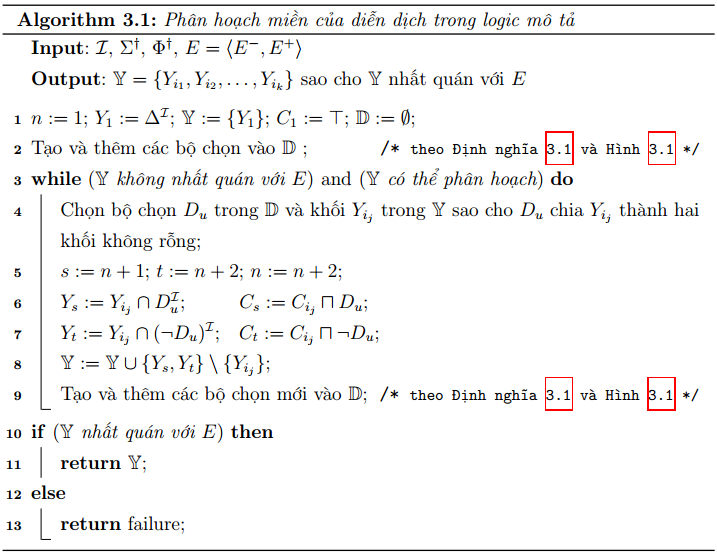
\includegraphics[scale=0.50]{ThuatToan1.png}
\end{frame}

%--------------------------------------------------------------------------
\begin{frame}\frametitle{\bf Học khái niệm trong logic mô tả}
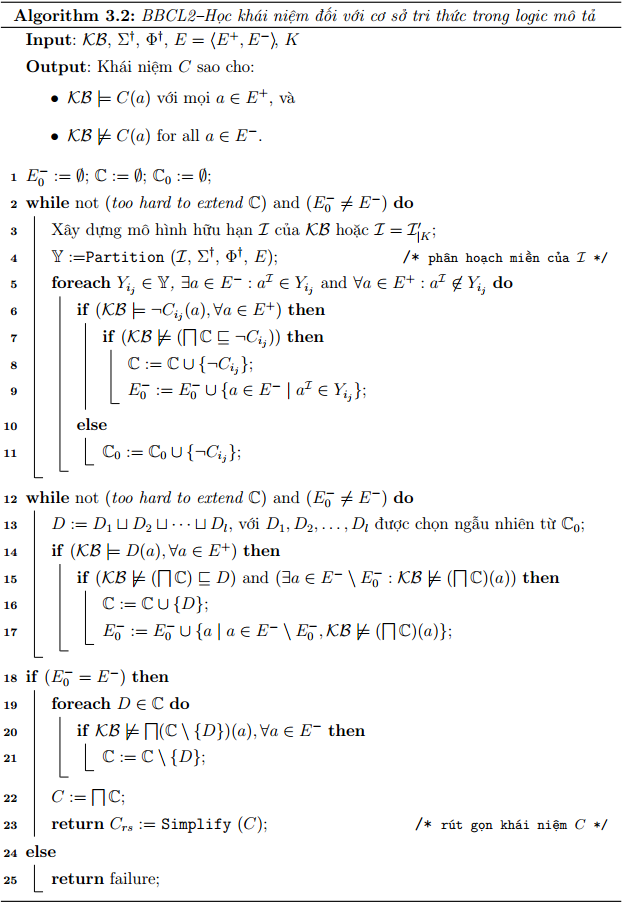
\includegraphics[scale=0.35]{ThuatToan2.png}
\end{frame}

%--------------------------------------------------------------------------
\begin{frame}\frametitle{\bf Học khái niệm trong logic mô tả}
\textbf{Tính đúng đắn của thuật toán \BBCLearnS}
\vspace{1.0ex}
	
	Thuật toán \BBCLearnS là đúng đắn. Nghĩa là, nếu thuật toán \BBCLearnS trả về một khái niệm $C_{rs}$ thì $C_{rs}$ là một lời giải của bài toán học khái niệm cho cơ sở tri thức trong logic mô tả với ngữ cảnh~(2).
\vspace{2.0ex}

\textbf{Độ phức tạp của thuật toán \BBCLearnS}
\vspace{1.0ex}
\begin{itemize}
	\item Đối với vấn đề suy luận tự động, độ phức tạp của bài toán này là \EXPTIME-khó ngay cả đối với logic mô tả cơ bản \ALC. 
\vspace{1.0ex}
	
	\item Một cách tổng quát, bài toán kiểm tra tính thỏa trong logic mô tả thường là \EXPTIME-đầy đủ.
\vspace{1.0ex}
	
	\item Thuật toán BBCL2 sử dụng một vòng lặp tuyến tính có giới hạn là lực lượng của $C_0$ cho bài toán suy luận. Do đó, thuật toán này có độ phức tạp là hàm mũ (xét theo kích thước của $\KB$, $E^+$ và $E^-$ với giả thiết là $\SigmaDag$ cố định).
\end{itemize}
\end{frame}

%--------------------------------------------------------------------------
\begin{frame}\frametitle{\bf Kết luận}
	\begin{itemize}
		\item Xây dựng ngôn ngữ logic mô tả $\mLSP$ dựa trên ngôn ngữ \ALCreg với tập các đặc trưng mở rộng gồm $\mI$, $\mO$, $\mN$, $\mQ$, $\mF$, $\mU$, $\Self$. Ngoài ra ngôn ngữ được xây dựng còn cho phép sử dụng các thuộc tính (bao gồm thuộc tính rời rạc và liên tục) như là các phần tử cơ bản của ngôn ngữ nhằm mô tả các hệ thống thông tin phù hợp với thực tế hơn.
		
		\item Xây dựng mô phỏng hai chiều trên lớp các logic mở rộng đang nghiên cứu. Các định lý, bổ đề, hệ quả liên quan đến mô phỏng hai chiều và tính bất biến đối với mô phỏng hai chiều cũng được phát triển và chứng minh trên lớp các logic mở rộng này.
		
		\item Dựa vào mô phỏng hai chiều, xây dựng thuật toán phân hoạch miền của mô hình của cơ sở tri thức và xây dựng thuật toán \BBCLearnS để học khái niệm trong logic mô tả cho cơ sở tri thức với ngữ cảnh~(2).
	\end{itemize}
\end{frame}
%--------------------------------------------------------------------------
\begin{frame}\frametitle{\bf Sản phẩm}
\begin{itemize}
	\item Hướng dẫn 01 luận văn Thạc sĩ chuyên ngành KHMT\\
	(Người hướng dẫn: TS. Hoàng Thị Lan Giao, thành viên).
	\vspace{1.5ex}
	\item Hướng dẫn 02 khóa luận Tốt nghiệp Đại học ngành Tin học\\
	(Người hướng dẫn: ThS. Trần Thanh Lương, chủ trì).
	\vspace{1.5ex}
	\item Công bố 04 bài báo trên các tạp chí/hội thảo khoa học trong nước và quốc tế.
	\vspace{1.5ex}
	\item Báo cáo đề tài.
\end{itemize}
\end{frame}
%--------------------------------------------------------------------------

\begin{frame}{}
\begin{center}
  \large{\textbf{EM XIN CẢM ƠN SỰ THAM DỰ CỦA THẦY CÔ}}
\end{center}
\end{frame}

\end{document}